\documentclass[tikz,border=8pt]{standalone}
\usepackage{amsmath}
\usepackage[scaled=0.95]{helvet}
\renewcommand{\familydefault}{\sfdefault}
\usetikzlibrary{arrows.meta,calc,positioning}

\definecolor{BaylorGreen}{HTML}{154734}
\definecolor{ModeRed}{HTML}{FF0000}
\definecolor{ModeGreen}{HTML}{008000}
\definecolor{ModeBlue}{HTML}{0000FF}
\definecolor{TensorFront}{HTML}{EEF3F0}
\definecolor{TensorTop}{HTML}{DCE8E2}
\definecolor{TensorSide}{HTML}{C9DBD2}
\definecolor{CalloutFill}{HTML}{F2F7F4}


\begin{document}
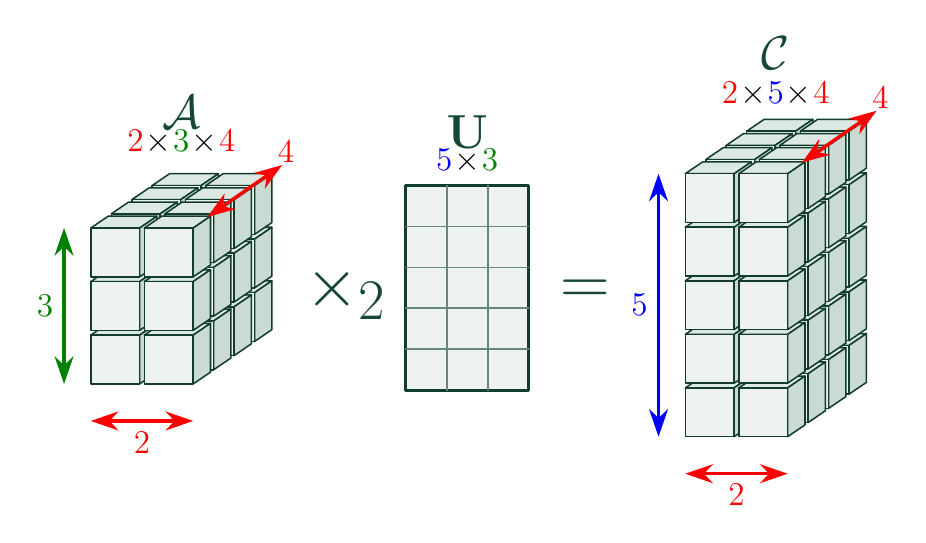
\begin{tikzpicture}[
  line cap=round,
  line join=round,
  >={Stealth[length=3.5mm,width=2.4mm]},
  dimension/.style={very thick,<->},
  cell edge/.style={draw=BaylorGreen!85!black,line width=0.55pt},
  matrix grid/.style={draw=BaylorGreen!65,line width=0.65pt},
  label text/.style={font=\large\bfseries},
  every node/.style={text=black}
]

% A slightly separated oblique cube. Repeating these makes every tensor
% entry visible as an individual unit while preserving the three modes.
\def\CubeW{0.62}
\def\CubeH{0.62}
\def\DepthX{0.22}
\def\DepthY{0.15}
\def\StepX{0.68}
\def\StepY{0.68}
\def\StepZX{0.26}
\def\StepZY{0.18}

\newcommand{\DrawVoxel}[2]{%
  \begin{scope}[shift={(#1,#2)}]
    \path[fill=TensorTop,cell edge]
      (0,\CubeH) -- (\DepthX,{\CubeH+\DepthY})
      -- ({\CubeW+\DepthX},{\CubeH+\DepthY})
      -- (\CubeW,\CubeH) -- cycle;
    \path[fill=TensorSide,cell edge]
      (\CubeW,0) -- ({\CubeW+\DepthX},\DepthY)
      -- ({\CubeW+\DepthX},{\CubeH+\DepthY})
      -- (\CubeW,\CubeH) -- cycle;
    \path[fill=TensorFront,cell edge] (0,0) rectangle (\CubeW,\CubeH);
  \end{scope}%
}

% Input tensor A: 2 x 3 x 4 = 24 visible units.
\def\Ax{0}
\def\Ay{0.72}
\foreach \k in {3,2,1,0} {
  \foreach \j in {0,1,2} {
    \foreach \i in {0,1} {
      \pgfmathsetmacro{\vx}{\Ax+\i*\StepX+\k*\StepZX}
      \pgfmathsetmacro{\vy}{\Ay+\j*\StepY+\k*\StepZY}
      \DrawVoxel{\vx}{\vy}
    }
  }
}

\node[font=\LARGE\bfseries,text=BaylorGreen] at (1.15,4.17) {$\mathcal A$};
\node[font=\large] at (1.15,3.79)
  {$\textcolor{ModeRed}{2}\!\times\!\textcolor{ModeGreen}{3}
    \!\times\!\textcolor{ModeRed}{4}$};

% Input dimensions.
\draw[dimension,ModeRed] (0,0.25) -- (1.30,0.25)
  node[midway,below,label text,text=ModeRed] {$2$};
\draw[dimension,ModeGreen] (-0.34,0.72) -- (-0.34,2.70)
  node[midway,left,label text,text=ModeGreen] {$3$};
\draw[dimension,ModeRed] (1.48,2.84) -- (2.43,3.50)
  node[pos=0.72, above right=3pt,label text, text=ModeRed] {$4$};

% Mode-product symbol.
\node[font=\Huge\bfseries,text=BaylorGreen] at (3.24,1.88) {$\times_{2}$};

% Matrix U: 5 x 3.
\def\Ux{4.00}
\def\Uy{0.64}
\def\UCell{0.52}
\path[fill=TensorFront,draw=BaylorGreen!85!black,line width=1.0pt]
  (\Ux,\Uy) rectangle ({\Ux+3*\UCell},{\Uy+5*\UCell});
\foreach \i in {1,2} {
  \draw[matrix grid] ({\Ux+\i*\UCell},\Uy)
    -- ({\Ux+\i*\UCell},{\Uy+5*\UCell});
}
\foreach \j in {1,2,3,4} {
  \draw[matrix grid] (\Ux,{\Uy+\j*\UCell})
    -- ({\Ux+3*\UCell},{\Uy+\j*\UCell});
}
\node[font=\LARGE\bfseries,text=BaylorGreen] at (4.78,3.92) {$\mathbf U$};
\node[font=\large] at (4.78,3.55)
  {$\textcolor{ModeBlue}{5}\!\times\!\textcolor{ModeGreen}{3}$};

\node[font=\Huge\bfseries,text=BaylorGreen] at (6.28,1.88) {$=$};

% Output tensor C: 2 x 5 x 4 = 40 visible units.
\def\Cx{7.55}
\def\Cy{0.05}
\foreach \k in {3,2,1,0} {
  \foreach \j in {0,1,2,3,4} {
    \foreach \i in {0,1} {
      \pgfmathsetmacro{\vx}{\Cx+\i*\StepX+\k*\StepZX}
      \pgfmathsetmacro{\vy}{\Cy+\j*\StepY+\k*\StepZY}
      \DrawVoxel{\vx}{\vy}
    }
  }
}

\node[font=\LARGE\bfseries,text=BaylorGreen] at (8.70,4.92) {$\mathcal C$};
\node[font=\large] at (8.70, 4.4)
  {$\textcolor{ModeRed}{2}\!\times\!\textcolor{ModeBlue}{5}
    \!\times\!\textcolor{ModeRed}{4}$};

% Output dimensions.
\draw[dimension,ModeRed] (7.55,-0.42) -- (8.85,-0.42)
  node[midway,below,label text,text=ModeRed] {$2$};
\draw[dimension,ModeBlue] (7.21,0.05) -- (7.21,3.39)
  node[midway,left,label text,text=ModeBlue] {$5$};
\draw[dimension,ModeRed] (9.03,3.53) -- (9.98,4.19)
  node[pos=0.72,above right=3pt,label text,text=ModeRed] {$4$};


\end{tikzpicture}
\end{document}
